\chapter{Training Neural Networks}

\section{What We'll Learn}

Having a conceptual framework for neural networks is important, but so is actually training the models. In this lesson, we will learn how to:

\begin{itemize}
    \item Distinguish between underfitting and overfitting
    \item Visualize our training with TensorBoard
    \item Optimize the training process with early stopping, regularization, dropout, random restarts, learning rate decay, and momentum
    \item Use PyTorch to build and train a neural network
\end{itemize}

\section{Training, Validation, and Testing}
\href{https://www.youtube.com/watch?v=HWt6gu5f3Q4&ab_channel=Udacity}{Youtube}\newline

\begin{itemize}
    \item Divide data to provide more information
    \begin{itemize}
        \item \textbf{Training}: Data actually used to fit model
        \item \textbf{Validation}: Data used during training to evaluate generalization. The validation dataset provides a lot of influence on the model since it informs how the model is likely to performs on the test data. This means it is a good leading indication for whether or not we have a problem with our data.
        \item Test: Data used to evaluate final model. Test data should be completely separated from the training and validation datasets. 
    \end{itemize}
\end{itemize}

\subsection{Dividing Data}

We typically divide our data into three sets whose size can vary, but a good rule of thumb is the 80/10/10 rule:

\begin{itemize}
    \item Train (80\%)
    \item Validation (10\%)
    \item Test (10\%)
\end{itemize}
Another powerful approach is k-fold cross-validation, where the data is split up into some number, which we call k, equal parts. One is used as the validation set, one is used as the test set, and the remaining parts are used as the training set. We then cycle through all combinations of the data until all parts have had a chance to be the test set.

\section{Overfitting and Underfitting}
\href{https://www.youtube.com/watch?v=xj4PlXMsN-Y&ab_channel=Udacity}{Youtube} \newline

When we train our models, it is entirely possible to get them to a point where they perform very well on our training data—but then perform very poorly on our testing data. Two common reasons for this are \textbf{underfitting} and \textbf{overfitting}

\subsection{Underfitting}

\begin{itemize}
    \item Underfitting means that our model is too simplistic. There is a poor fit between our model and the data because we have \textbf{oversimplified} the problem.
    \item Underfitting is sometimes referred to as \textbf{error due to bias}. Our training data may be biased and this bias may be incorporated into the model in a way that oversimplifies it.
\end{itemize}
For example, suppose we train an image classifier to recognize dogs. And suppose that the only type of animal in the training set is a dog. Perhaps the model learns a biased and overly simple rule like, "if it has four legs it is a dog". When we then test our model on some data that has other animals, it may misclassify a cat as a dog—in other words, it will \textit{underfit} the data because it has \textit{error due to bias}.

\subsection{Overfitting}

\begin{itemize}
    \item Overfitting means that our model is too complicated. The fit between our model and the training data is \textbf{too specific}—the model will perform very well on the training data but will \textbf{fail to generalize} to new data.
    \item Overfitting is sometimes referred to as \textbf{error due to variance}. This means that there are random or irrelevant differences among the data points in our training data and we have fit the model so closely to these irrelevant differences that it performs poorly when we try to use it with our testing data.
\end{itemize}
For example, suppose we want our image classifier to recognize dogs, but instead we train it to recognize "dogs that are yellow, orange, or grey." If our testing set includes a dog that is brown, for example, our model will put it in a separate class, which was not what we wanted. Our model is too specific—we have fit the data to some unimportant differences in the training data and now it will fail to generalize.

\subsection{Applying This to Neural Networks}

Generally speaking, underfitting tends to happen with neural networks that have overly simple architecture, while overfitting tends to happen with models that are highly complex.

\includegraphics[width=0.75\linewidth]{img//intro//trainingNN/training-considerations-3.png}

The bad news is, it's really hard to find the right architecture for a neural network. There is a tendency to create a network that either has overly simplistic architecture or overly complicated architecture. In general terms, the approach we will take is to err on the side of an overly complicated model, and then we'll apply certain techniques to reduce the risk of overfitting.

\includegraphics[width=0.75\linewidth]{img//intro//trainingNN/image.png}

\section{Early Stopping}
\href{https://www.youtube.com/watch?v=NnS0FJyVcDQ&t=2s&ab_channel=Udacity}{Youtube} \newline

When training our neural network, we start with random weights in the first epoch and then change these weights as we go through additional epochs. Initially, we expect these changes to improve our model as the neural network fits the training data more closely. But after some time, further changes will start to result in overfitting.

\includegraphics[width=1\linewidth]{img//intro//trainingNN/training-considerations-4.png}

We can monitor this by measuring both the \textbf{training error} and the \textbf{testing error}. As we train the network, the training error will go down—but at some point, the testing error will start to increase. This indicates overfitting and is a signal that we should stop training the network prior to that point. We can see this relationship in a \textbf{model complexity graph} like this one:

\includegraphics[width=1\linewidth]{img//intro//trainingNN/training-considerations-5.png}

\includegraphics[width=1\linewidth]{img//intro//trainingNN/early-stopping.png}
\captionof{figure}{Model complexity graph}

Have a look at the graph and make sure you can recognize the following:

\begin{itemize}
    \item On the Y-axis, we have a measure of the error and on the X-axis we have a measure of the complexity of the model (in this case, it's the number of epochs).
    \item On the left we have high testing and training error, so we're underfitting.
    \item On the right, we have high testing error and low training error, so we're overfitting.
    \item Somewhere in the middle, we have our happy Goldilocks point (the point that is "just right").
\end{itemize}
In summary, we do gradient descent until the testing error stops decreasing and starts to increase. At that moment, we stop. This algorithm is called \textbf{early stopping} and is widely used to train neural networks.


\section{Visualizing Training with Tensorboard}
\href{https://www.youtube.com/watch?v=MKoW6vUYStk&t=1s&ab_channel=Udacity}{Youtube} \newline

After launching Tensorboard from the command line and choosing a directory for the logs, we use the \verb|SummaryWriter| class from \verb|torch.utils.tensorboard|. Using the \verb|add_scalar| method, we can write things like loss and accuracy. We can also put images and figures into Tensorboard using \verb|add_image| and \verb|add_figure| respectively. \newline

For further information, check the \href{https://pytorch.org/docs/stable/tensorboard.html}{\textbf{PyTorch Tensorboard documentation}}

\section{Regularization}
\href{https://www.youtube.com/watch?v=KxROxcRsHL8&ab_channel=Udacity}{Youtube} \newline

Consider a situation where we are attempting to split two points, and have two possible models that could be used. We are trying to find the model with the smallest error.

\includegraphics[width=0.75\linewidth]{img//intro//trainingNN/image2.png}

A couple of reminders:
\begin{itemize}
    \item The prediction is: \(\hat{y} = \sigma(w_1 x_1 + w_2 x_2 + b)\)
    \item The general equation for a linear model is: \(w_1 x_1 + w_2 x_2 + b = 0\)
\end{itemize}

\textbf{Solution 1}: \(x_1 + x_2\)\newline
Notice that the bias \(b\) is \(0\) and \(w_1\) and \(w_2\) are both equal to \(1\).
\begin{itemize}
    \item \(\sigma(1 + 1) = 0.88\)
    \item \(\sigma(-1 + -1) = 0.12\)
\end{itemize}

\textbf{Solution 2}: \(10x_1 + 10x_2\)
\begin{itemize}
    \item \(\sigma(10 + 10) = 0.9999...\)
    \item \(\sigma(-10 + -10) = 0.000000...2\)
\end{itemize}

\textbf{Solution}: \(10x_1 + 10x_2\). The error is smaller if the prediction is closer to the actual label. Great intuition about the error function! \href{https://www.youtube.com/watch?v=ndYnUrx8xvs&t=66s&ab_channel=Udacity}{Youtube}\newline

But, the model is overfit in a subtle way. The sigmoid functions for the two models are shown in \ref{fig:activationFunc} and as shown, the second solution is too certain and its sigmoid function is too steep. As a result, it is much harder to do gradient descent since the derivatives are mostly close to 0, except where it crosses the y-axis and becomes very large. It is difficult to train under these circumstances. Hence, we would prefer to have a model as on the left.

\includegraphics[width=1\linewidth]{img//intro//trainingNN/actibation-functions.png}
\captionof{figure}{Activation functions}
\label{fig:activationFunc}


\begin{itemize}
    \item When we apply sigmoid to small values such as \(x_1 + x_2\), we get the function on the left, which has a nice slope for gradient descent.
    \item When we multiply the linear function by 10 and take sigmoid of \(10 x_1 + 10 x_2\), our predictions are much better since they're closer to zero and one. But the function becomes much steeper and it's much harder to do gradient descent.
\end{itemize}
Conceptually, the model on the right is too certain and it gives little room for applying gradient descent. Also, the points that are classified incorrectly in the model on the right will generate large errors and it will be hard to tune the model to correct them. \newline

Now the question is, how do we prevent this type of overfitting from happening? The trouble is that large coefficients are leading to overfitting, so what we need to do is adjust our error function by, essentially, penalizing large weights. \newline

If you recall, our original error function looks like this: \[-\frac{1}{m} \sum_{i = 1}^m (1 - y_i) \ln{(1 - \hat{y}_i)} + y_i \ln{(\hat{y}_i)}\]
We want to take this and add a term that is big when the weights are big. There are two ways to do this. One way is to add the sums of absolute values of the weights times a constant lambda: \[+ \lambda(|w_i| + ... + |w_n|)\]

The other one is to add the sum of the squares of the weights times that same constant: \[+ \lambda (w_1^2 + ... + w_n^2)\]

In both cases, these terms are large if the weights are large.

\includegraphics[width=1\linewidth]{img//intro//trainingNN/training-considerations-9.png}

\subsection{L1 vs L2 Regularization}

The first approach (using absolute values) is called \textbf{L1 regularization}, while the second (using squares) is called \textbf{L2 regularization}. Here are some general guidelines for deciding between the two:

\subsubsection{L1 Regularization}

\begin{itemize}
    \item L1 tends to result in sparse vectors. That means small weights will tend to go to zero.
    \item If we want to reduce the number of weights and end up with a small set, we can use L1.
    \item L1 is also good for feature selection. Sometimes we have a problem with hundreds of features, and L1 regularization will help us select which ones are important, turning the rest into zeroes.
\end{itemize}

\subsubsection{L2 Regularization}

\begin{itemize}
    \item L2 tends not to favor sparse vectors since it tries to maintain all the weights homogeneously small.
    \item L2 gives better results for training models so it's the one we'll use the most.
\end{itemize}

\includegraphics[width=0.75\linewidth]{img//intro//trainingNN/training-considerations-10.png}

\section{Implementing Regularization}\label{implementing-regularization}

In this exercise, you will implement both L1 and L2 regularization from
scratch in NumPy. In PyTorch, L2 regularization is typically handled in
the optimizer, via the \lstinline!weight\_decay!
parameter, but we will also implement a manual L1 and L2 loss penalty in
PyTorch.

\begin{lstlisting}[language=Python]
# DO NOT EDIT THIS CELL
import numpy as np
import torch
from torch import nn
from torch import optim
import torch.nn.functional as F
from torch.utils.data import DataLoader
from torchvision import transforms
from torchvision import datasets
import matplotlib.pyplot as plt
\end{lstlisting}

\subsection{L1 Regularization -- Numpy}\label{l1-regularization-numpy}

L1 regularization is the sum of the absolute values of the weights times
a scaling constant, lambda. Below, you will define the function
\lstinline!l1\_regularization! that accepts an input
vector and a scalar constant, lambda.

\textbf{NOTE:} We use the variable name \lstinline!lamb!
rather than \lstinline!lambda! since
\lstinline!lambda! is a keyword in Python.

\begin{lstlisting}[language=Python]
def l1_regularization(weights, lamb):
    absolute_weights = np.abs(weights)
    return lamb * np.sum(absolute_weights)
\end{lstlisting}

\begin{lstlisting}[language=Python]
# Grading code. Run this cell to test your code!
grading_vector = np.array([1, -2, 3, -4])
assert l1_regularization(grading_vector, 0.5) == 5, f"Your L1 regularization implementation seems to be incorrect. Expected 5, got {l1_regularization(grading_vector, 0.5)}"
assert l1_regularization(grading_vector, 1) == 10, f"Your L1 regularization implementation seems to be incorrect. Expected 10, got {l1_regularization(grading_vector, 1)}"

print("Great work!")
\end{lstlisting}

\begin{lstlisting}
Great work!
\end{lstlisting}

\subsection{L2 Regularization -- Numpy}\label{l2-regularization-numpy}

L2 regularization squares the weights inside the vector and returns the
sum of those squares times a scaling constant, lambda. Below, you will
define the function \lstinline!l2\_regularization!, which
accepts an input vector and a scalar constant, lambda.

\begin{lstlisting}[language=Python]
def l2_regularization(weights, lamb):
    squared_weights = np.dot(weights, weights.T)
    return lamb * squared_weights
\end{lstlisting}

\begin{lstlisting}[language=Python]
# Grading code. Run this cell to test your code!
grading_vector = np.array([0.5, -1, 1.5, -2])
assert l2_regularization(grading_vector, 0.5) == 3.75, f"Your L2 regularization implementation seems to be incorrect. Expected 3.75, got {l2_regularization(grading_vector, 0.5)}"
assert l2_regularization(grading_vector, 1) == 7.5, f"Your L2 regularization implementation seems to be incorrect. Expected 7.5, got {l2_regularization(grading_vector, 1)}"

print("Great work!")
\end{lstlisting}

\begin{lstlisting}
Great work!
\end{lstlisting}

\subsection{Regularization in PyTorch}\label{regularization-in-pytorch}

Although L2 regularization is typically handled via the
\lstinline!weight\_decay! parameter in your optimizer, we
can compute L1 and L2 regularization by hand. We do this by iterating
over the parameters in our model using the
\lstinline!net.parameters()! method.

Rather than establishing a model, training it, and testing it, we will
manually set the model weights.

\begin{lstlisting}[language=Python]
# Setting up our net for testing
net = nn.Sequential(nn.Linear(4, 1, bias=False))
# Make it so autograd doesn't track our changes
with torch.no_grad():
    net[0].weight = nn.Parameter(torch.ones_like(net[0].weight))
    net[0].weight.fill_(2.0)
\end{lstlisting}

\begin{lstlisting}[language=Python]
# Define L1 loss
def l1_torch(model, lamb):
    return lamb * sum([p.abs().sum() for p in model.parameters()])

# Define L2 loss
def l2_torch(model, lamb):
    return lamb * sum([(p**2).sum() for p in model.parameters()])
\end{lstlisting}

\begin{lstlisting}[language=Python]
# Grading code
assert l1_torch(net, 1) == 8, f"There is something wrong with your L1 regularization implementation. Expected 8, got {l1_torch(net, 1)}"
assert l1_torch(net, 0.5) == 4, f"There is something wrong with your L1 regularization implementation. Expected 4, got {l1_torch(net, 0.5)}"

assert l2_torch(net, 1) == 16, f"There is something wrong with your L2 regularization implementation. Expected 16, got {l2_torch(net, 1)}"
assert l2_torch(net, 0.25) == 4, f"There is something wrong with your L2 regularization implementation. Expected 4, got {l2_torch(net, 0.25)}"

print("Great work!")
\end{lstlisting}

\begin{lstlisting}
Great work!
\end{lstlisting}

\begin{lstlisting}[language=Python]
\end{lstlisting}



\section{Dropout}
\href{https://www.youtube.com/watch?v=Ty6K6YiGdBs&ab_channel=Udacity}{Youtube} \newline

When training a neural network, sometimes one part of the network has very large weights and it ends up dominating the training, while another part of the network doesn't really play much of a role (so it doesn't get trained).

To solve this, we can use a method called \textbf{dropout} in which we turn part of the network off and let the rest of the network train:

\begin{itemize}
    \item We go through the epochs and randomly turn off some of the nodes. This forces the other nodes to pick up the slack and take a larger part in the training.
    \item To drop nodes, we give the algorithm a parameter that indicates the probability that each node will get dropped during each epoch. For example, if we set this parameter to 0.2, this means that during each epoch, each node has a 20\% probability of being turned off.
    \item Note that some nodes may get turned off more than others and some may never get turned off. This is OK since we're doing it over and over; on average, each node will get approximately the same treatment.
\end{itemize}

\section{Local Minima and Random Restart}
\href{https://www.youtube.com/watch?v=gF_sW_nY-xw&t=1s&ab_channel=Udacity}{Youtube} \newline
Gradient descent looks at the direction where it can most decrease the error and then it takes a step in that direction. However, if there are multiple low points in the solution space, gradient descent may end up leading us to \textbf{local minima}—solutions where the error is at the lowest point in the local area, but not the lowest point overall.

\includegraphics[width=0.75\linewidth]{img//intro//trainingNN/training-considerations-13.png}

One way to solve our problem is to use \textbf{random restart}. We start (and restart) from a few different random places and do gradient descend from all of them. This increases the probability that we'll get to the global minimum, or at least a pretty good local minimum. 

\includegraphics[width=0.75\linewidth]{img//intro//trainingNN/training-considerations-15.png}

\href{https://www.youtube.com/watch?v=idyBBCzXiqg&t=1s&ab_channel=Udacity}{Youtube on random restart}


\section{Exercise: Training Techniques}

\subsection{Scenario 1:}

You are training a neural network and see the following accuracy and loss in TensorBoard:

\includegraphics[width=1\linewidth]{img//intro//trainingNN/screen-shot-2022-04-10-at-7.01.14-am.jpeg}

Based on the screenshot, what is happening to your model?

(Select all that apply.)

\begin{itemize}
    \item It is underfitting to the training set
    \item \textbf{It is overfitting to the training set}
    \item \textbf{It is stuck in a local minimum}
    \item It has not trained long enough
\end{itemize}
Solution: This model has gotten stuck in a local minimum very quickly and vastly overfit the training set.

Which \textbf{two} of the following techniques would be most helpful for this scenario?
\begin{itemize}
    \item Training for more epochs
    \item \textbf{Early stopping}
    \item \textbf{Random restart}
    \item Dropout
\end{itemize}
Solution: Early stopping will help us with our overfitting problem and random restart can help us escape the local minimum.


\subsection{Scenario 2:}

You're training another neural network and find the following accuracy and loss in TensorBoard:

\includegraphics[width=1\linewidth]{img//intro//trainingNN/screen-shot-2022-04-10-at-7.44.41-am.jpeg}

Which of the following is occurring?
\begin{itemize}
    \item \textbf{The model is not sufficiently trained}
    \item The model is underfit to the training set
    \item The model is overfit to the training set
    \item The model is stuck in a local minimum
\end{itemize}
Solution: Looking carefully also shows that our learning rate is probably too low. Underfitting and undertraining can look very similar, but underfitting means that the model is too simple, not that it hasn't trained long enough. We can see that the loss is still decreasing at a similar rate each epoch -- it hasn't leveled off.

\section{Vanishing and Exploding Gradients}
\href{https://www.youtube.com/watch?v=ff3GFgnE4PU&t=62s&ab_channel=Udacity}{Youtube} \newline

\subsection{Vanishing gradients}
\textbf{Vanishing gradients} are common for certain activation function with limited range. These are also called \textbf{"saturating" activation functions}. This means that as error back backpropagates through the model, the error signal becomes weaker. Ths is more common in deeper neural networks. 

We have our output neuron which gives our loss. We then compute that error and backpropagate the error through the network. The input to the output neuron is going to consist of the input from the prior hidden layer. So the relative contribution to the neuron highlighted in blue (right after the output error on the right side of \autoref{fig:vanishingGradient2}) is the product of the partial derivative of the loss with respect to the weight of the blue neuron, and the error signal sent back to that is going to be a little smaller than the overall signal since it is split between the inputs. 

\includegraphics[width=0.75\linewidth]{img//intro//trainingNN/image2.png}
\captionof{figure}{ }
\label{fig:vanishingGradient2}

Because of how backpropagation works via the chain rule, the error sent to the neuron in the last hidden layer is that partial derivative with respect to the weight of the neuron and the prior layer. And this is again going to be a bit smaller. 

\includegraphics[width=1\linewidth]{img//intro//trainingNN/image3.png}

This signal has to travel all the way back through the network. So if the gradient is relatively small to begin with, we are multiplying progressively smaller numbers between \(0\) and \(1\) by each other, causing our gradient to completely vanish by the time it reaches the earliest layers. 

This problem can be solved by using non-saturating activation functions like ReLU.  However, function like ReLu contribute e to different problems: the \textbf{exploding gradients}.

\subsection{Exploding gradients}
The exploding gradients are more common in deeper networks as there are more opportunities for these gradients to be multiplied against each other. These are common for non-saturating activation functions like ReLU. These function are unbounded so their gradients can easily be greater than \(1\).  \newline

We want to backpropagate the error through the model. Assuming the gradient of the error with respect to that top neuron is reasonably sized, but greater than \(1\). Then the gradient with respect to each preceding layer is going to be the product of all the preceding gradients. So if the gradients are larger than one (for these non-saturating activation functions, they can be significantly larger than \(1\)), the gradient will grow exponentially larger and can \textbf{explode}. \newline

This causes instability and makes it hard to train a model. 
\subsection{How to know}
Watch weights of neurons on TensorBoard. \newline

Vanishing gradient: Weights of neurons drop to 0 but loss is relatively high but stalled. \newline

Exploding gradient: Neuron weights become very large during training. Loss is unstable. It can jump significantly from epoch to epoch and possibly even going to NaN.

\includegraphics[width=0.75\linewidth]{image.png}

To solve either of them, consider changing the activation function.  For exploding gradients, consider gradient clipping or weight regularization.

\subsection{Quiz Question}

Consider the six activation functions depicted above. Which of the six are most susceptible to \textit{vanishing} gradients?

*\textit{Select all that apply}

\begin{itemize}
    \item ReLU
    \item Leaky ReLu
    \item \textbf{Sigmoid}
    \item \textbf{tanh}
    \item \textbf{Step}
    \item GELU

\end{itemize}


\subsection{Quiz Question}

In addition to changing the activation function, we can use the \href{https://pytorch.org/docs/stable/generated/torch.nn.utils.clip_grad_norm_.html}{\textbf{\lstinline{torch.nn.utils.clip_grad_norm_}}} function to clip our gradients. What effect will this have?
\begin{itemize}
    \item \textbf{Prevent exploding gradients by bound the norm of the gradient}
    \item Prevent vanishing gradients by adding noise to the gradient
    \item Prevent exploding gradients by bounding the value of the gradient
    \item PRevent vanishing gradients by setting a minimum gradient size
\end{itemize}
Solution: We can also use the \href{https://pytorch.org/docs/stable/generated/torch.clamp.html#torch.clamp}{\textbf{\lstinline{clamp}}} method to restrict the minimum and maximum size of our tensors.

\section{Learning Rate Decay}
\href{https://www.youtube.com/watch?v=TwJ8aSZoh2U&ab_channel=Udacity}{Youtube} \newline

Here are some key ideas to keep in mind when choosing a \textbf{learning rate}:

If the learning rate is \textbf{large}:

\begin{itemize}
    \item This means the algorithm is taking large steps, which can make it faster.
    \item However, the large steps may cause it to miss (overshoot) the minimum.
\end{itemize}
If the learning learning rate is \textbf{small}:

\begin{itemize}
    \item This means the algorithm is taking small steps, which can make it slower.
    \item However, it will make steady progress and have a better chance of arriving at the local minimum.
\end{itemize}
If your model is not working, a good general rule of thumb is to try decreasing the learning rate. The best learning rates are those that decrease as the algorithm is getting closer to a solution.

\includegraphics[width=1\linewidth]{img//intro//trainingNN/training-considerations-26.png}

\section{Momentum}
\href{https://www.youtube.com/watch?v=r-rYz_PEWC8&t=1s&ab_channel=Udacity}{Youtube} \newline
 
Another way to solve the local minimum problem is with \textbf{momentum}. In the analogy, this would mean walking quickly and with momentum to “power through” small increases in the error function, so that a lower minimum can be found. Momentum is a constant \(\beta\) between \(0\) and \(1\). \newline

We use \(\beta\) to get a sort of weighted average of the previous steps: \[{step}(n) + \beta {step}(n - 1) + \beta^2{step}(n) + \beta^3{step}(n - 2) + ...\]

\includegraphics[width=1\linewidth]{img//intro//trainingNN/image4.png}

The previous step gets multiplied by \(1\), the one before it gets multiplied by \(\beta\), the one before that by \(\beta^2\), the one before that by \(\beta^3\), and so on. Because \(\beta\) has a value between \(0\) and \(1\), raising it to increasingly large powers means that the value will get smaller and smaller. In this way, the steps that happened a long time ago will be multiplied by tiny values and thus matter less than the ones that happened recently.\newline

This can get us over "humps" and help us discover better minima. Once we get to the global minimum, the momentum will still be pushing us away, but not as much.


\section{Optimizers}
\href{https://www.youtube.com/watch?v=4Ocl-2lwO6U&t=1s&ab_channel=Udacity}{Youtube} \newline

We want to change weight to minimize error. Gradient descent is an optimization algorithm that works for many but not all problems since it does not incorporate things like learning rate or momentum. One of the most common optimizers for NN is Adaptive Moment Estimation (Adam).  \newline

With Adam, the learning rate does not vanish and it quickly converges to a minimum.  

\subsection{Choosing an Optimizer}

Our choice of optimizer is not often the most important decision in training a model, but it can definitely make a difference. While Adam is a good default, the use of SGD is still common. The various optimizers available in PyTorch are covered in \href{https://pytorch.org/docs/stable/optim.html}{\textbf{the \lstinline{torch.optim} documentation}}

\subsection{Quiz Question}

What parameter of the Adam optimizer tells it how big of a step to take when we call the \verb|.step()| method?

You can reference \href{https://pytorch.org/docs/stable/generated/torch.optim.Adam.html\#torch.optim.Adam}{\textbf{the documentation}} if you get stuck.
\begin{itemize}
    \item \lstinline{params}
    \item \textbf{\lstinline{lr}}
    \item \lstinline{betas}
    \item \lstinline{weight_decay}
\end{itemize}
Solution: The learning rate is a very important parameter for our optimizer. If we set it too small, training may not converge. Setting the learning rate too high can cause the optimizer to overshoot the global minimum.

\section{Batch vs Stochastic Gradient Descent}
\href{https://www.youtube.com/watch?v=2p58rVgqsgo&t=1s&ab_channel=Udacity}{Youtube}
\subsection{Batch Gradient Descent}

First, let's review our \textbf{batch gradient descent} algorithm:

\begin{itemize}
    \item In order to decrease error, we take a bunch of steps following the negative of the gradient, which is the error function.
    \item Each step is called an \textit{epoch}.
    \item In each epoch, we take our input (all of our data) and run it through the entire neural network.
    \item Then we find our predictions and calculate the error (how far the predictions are from the actual labels).
    \item Finally, we back-propagate this error in order to update the weights in the neural network. This will give us a better boundary for predicting our data.
\end{itemize}
If we have a large number of data points then this process will involve huge matrix computations, which would use a lot of memory.

\subsection{Stochastic Gradient Descent}

To expedite this, we can use only \textit{some} of our data at each step. If the data is well-distributed then a subset of the data can give us enough information about the gradient.

This is the idea behind \textbf{stochastic gradient descent}. We take small subsets of the data and run them through the neural network, calculating the gradient of the error function based on these points and moving one step in that direction.

We still want to use all our data, so what we do is the following:

\begin{itemize}
    \item Split the data into several batches.
    \item Take the points in the first batch and run them through the neural network.
    \item Calculate the error and its gradient.
    \item Back-propagate to update the weights (which will define a better boundary region).
    \item Repeat the above steps for the rest of the batches.
\end{itemize}
Notice that with this approach we take multiple steps, whereas with batch gradient descent we take only one step with all the data. Each step may be less accurate, but, in practice, it's much better to take a bunch of slightly inaccurate steps than to take only one good one.


\section{Training Techniques in PyTorch}
\href{https://www.youtube.com/watch?v=dmeeuBWa1us&t=1s&ab_channel=Udacity}{Youtube} \newline

When using PyTorch without API, early stopping has to be implemented by programmer. 

\subsection{Implementing Training Techniques in PyTorch}

The various training optimizations we've covered are relatively easy to implement when training our networks. Though early stopping is not written into PyTorch itself, implementing it in the training loop is fairly easy.

Our other techniques are more straightforward and can be found in the PyTorch documentation:

\begin{itemize}
    \item \href{https://pytorch.org/docs/stable/generated/torch.nn.Dropout.html}{\textbf{Dropout}}
    \item Momentum and learning rate decay are implemented in the \href{https://pytorch.org/docs/stable/optim.html}{\textbf{optimizer}}
\end{itemize}

\subsection{Writing Training Loops}
\href{https://www.youtube.com/watch?v=Ek3_IL-kt6Y&ab_channel=Udacity}{Youtube} 

To write a training loop, one typically begins with the \verb|for epoch in range(epochs)| syntax. Then, loading each batch from the dataloader, the steps of training are:

\begin{itemize}
    \item Zeroing out the optimizer's gradients with \verb|optimizer.zero_grad()|
    \item Computing the outputs with \verb|net(inputs)|
    \item Computing the loss with \verb|criterion(outputs, labels)|
    \item Computing the gradient of the loss with \verb|loss.backward()|
    \item Taking an update step with the optimizer using \verb|optimizer.step()|
\end{itemize}
We can also implement early stopping, compute validation loss and accuracy, and print updates in the training loop.

\section{Lesson Review}
At the beginning of this lesson, we needed to develop the skills to actually train a neural network using PyTorch. In this lesson, we learned how to:

\begin{itemize}
    \item Split our data into training, validation, and test sets
    \item Distinguish between and understand the causes of underfitting and overfitting
    \item Optimize the model training process with early stopping, regularization, and dropout
    \item Define a loss function and optimizer to train a neural network
    \item Write a training loop to use PyTorch to build a neural network
\end{itemize}
Using these skills, we can train a neural network from scratch and ensure that it generalizes well to unseen data.

\section{Glossary}

For your reference, here are all the new terms we introduced in this lesson:

\begin{itemize}
    \item \textbf{Training Data}: Data actually used to fit the model
    \item \textbf{Validation Data}: Data used during training to evaluate generalization
    \item \textbf{Test Data:} Data used to evaluate the final model
    \item \textbf{Underfitting} (also called error due to bias): Underfitting means that our model is too simplistic because of a poor fit between our model, and the data because we have oversimplified the problem.
    \item \textbf{Overfitting} (also called error due to variance)\textbf{:} Overfitting means that our model is too complicated, and the fit between our model and the training data is too specific—the model will perform very well on the training data but will fail to generalize to new data.
    \item \textbf{Early Stopping:} Implementing gradient descent until the testing error stops decreasing and starts to increase.
    \item \textbf{Dropout}: The process of turning part of the network off and letting the rest of the network train
    \item \textbf{Local Minima:} solutions where the error is at the lowest point in the local area, but not the lowest point overall.
    \item \textbf{Momentum:} Momentum is a constant \(\beta\) between 00 and 11.
    \item \textbf{Stochastic gradient descent}: The process of taking small subsets of the data and running them through the neural network, calculating the gradient of the error function based on these points, and moving one step in that direction.
\end{itemize}
